\chapter{Linguagens Regulares}
\label{cha:automatos}

Neste capítulo estudaremos um modelo simples de computação, os autômatos finitos, e a classe das linguagens regulares.

\section{Introdução}
\label{sec:linguagens-regulares}

Voltaremos nossa atenção um instante para conjuntos (classes) de linguagens, ou seja, conjuntos de conjuntos de strings.

\begin{example}
\begin{itemize}
\item[] $\L = \{A: A \subseteq \Sigma^*\}$ é o conjunto de todas as linguagens sobre $\Sigma$
\item[] $\emptyset$ é a classe vazia.
\item[] $\{\emptyset\}$ é a classe que contém apenas a linguagem vazia.
\item[] $\{\{\varepsilon\}, \emptyset\}$ é a classe que contém a linguagem vazia e a linguagem que possui apenas a string vazia.
\end{itemize}
\end{example}

Podemos aplicar operações sobre linguagens.
Como linguagens são conjuntos de strings, podemos tomar a {\em união} de duas linguagens:
\begin{displaymath}
  A \cup B = \{x \in \Sigma^* : x \in A \textrm{ ou } x \in B\}
\end{displaymath}


\begin{example}
  \begin{eqnarray*}
    A & = & \{p_1p_2, p_1, p_2p_1\}\\
    B & = & \{p_1p_1, p_3, p_1\}\\
    A \cup B & = & \{p_1p_2, p_1, p_2p_1, p_1p_1, p_3\}
  \end{eqnarray*}
\end{example}

Outra operação sobre linguagens é {\em concatenação} que consiste na concatenação de cada combinação de strings da linguagem:

\begin{displaymath}
  A \circ B = \{x \cdot y \in \Sigma^* : x \in A \textrm{ e } x \in B\}
\end{displaymath}

\begin{example}
  \begin{eqnarray*}
    A & = & \{p_1p_2, p_1\}\\
    B & = & \{p_1p_1, p_3\}\\
    A \circ B & = & \{p_1p_2p_1p_1, p_1p_2p_3, p_1p_1p_1, p_1p_3\}\\
    B \circ A & = & \{p_1p_1p_1p_2, p_1p_1p_1, p_3p_1p_2, p_3p_1\}\\
    A \circ A & = & \{p_1p_2p_1p_2, p_1p_2p_1, p_1p_1p_2, p_1p_1\}
  \end{eqnarray*}
\end{example}

Podemos, por fim, aplica a {\em estrela de Kleene} sobre uma linguagem para produzir todas as possíveis concatenações dos elementos:

\begin{displaymath}
  A^* = \{x_1 \dots x_k \in \Sigma^* : x_i \in A \}
\end{displaymath}


\begin{example}
  \begin{eqnarray*}
    A & = & \{a,b\}\\
    A^* & = & \{\varepsilon, a, b, aa, ab, bb, ba, aaa, aab, aba, abb, \dots\}
  \end{eqnarray*}
\end{example}

Repare que a notação $\Sigma^*$ é consistente com a definição de estrela de Kleene.

As operações de união, concatenação e estrela de Kleene sobre linguagens são chamadas {\em operações regulares}.

\begin{example}
  \begin{eqnarray*}
    A & = & \{a\}\\
    B & = & \{aa, b\}\\
    A \circ B & = & \{aaa, ab\}\\
    A \cup (A \circ B) & = & \{a, aaa, ab\}\\
    (A \cup (A \circ B))^* & = & \{\varepsilon, a, aaa, ab, aa, aaaa, aab, aaaaaa, aaaab, \dots \}\\
  \end{eqnarray*}
\end{example}

Uma classe de linguagens $\L$ é {\em fechada por união} quando temos que:
\begin{displaymath}
\textrm{se }  A, B \in \L \textrm{ então } A \cup B \in \L
\end{displaymath}

Analogamente, uma classe de linguagens $\L$ é {\em fechada por concatenação} quando temos que:
\begin{displaymath}
\textrm{se }  A, B \in \L \textrm{ então } A \circ B \in \L
\end{displaymath}

Por fim, $\L$ é {\em fechada pela estrela de Kleene} quando temos que:

\begin{displaymath}
\textrm{se }  A \in \L \textrm{ então } A^* \in \L
\end{displaymath}

\begin{example}
  \begin{eqnarray*}
    \L_1 & = & \{\{a\}, \{b\}\} \\
    \L_2 & = & \{\{a\}, \{b\}, \{a, b\}\}\\
    \L_3 & = & \{\{a\}, \{a, aa\}, \{a, aa, aaa\} \dots\}\\
    \L_4 & = & \{\{a\}, \{\varepsilon, a, aa, aaa, \dots\}\}\\
  \end{eqnarray*}

  $\L_1$ não é fechada por união, mas $\L_2$ é.
  $\L_3$ é fechada por concatenação e $\L_4$ é fechada pela estrela de Kleene.
\end{example}

A classe das {\em linguagens regulares} é a menor classe de linguagens fechada por união, concatenação e estrela de Kleene que contém a seguinte linguagem:
\begin{displaymath}
  \{\{a\} : a \in \Sigma\}
\end{displaymath}

Uma foram alternativa de definir linguagens regulares é por meio de expressões regulares.
Uma {\em expressão regular} pode ser definida da seguinte forma:
\begin{itemize}
\item[] se $r \in \Sigma$ então $r$ é uma expressão regular,
\item[] $\epsilon$ é uma expressão regular,
\item[] $\o$ é uma expressão regular,
\item[] se $r_1$ e $r_2$ são expressões regulares então $r_1 \abxcup r_2$ é uma expressão regular,
\item[] se $r_1$ e $r_2$ são expressões regulares então $r_1 r_2$ é uma expressão regular e
\item[] se $r$ é uma expressão regular então $r^\star$ é uma expressão regular.
\end{itemize}


\begin{example}
  São expressões regulares:
\begin{itemize}
\item[] $\o$
\item[] $01$
\item[] $01^\star\abxcup 1$
\item[] $\epsilon \abxcup \o$
\end{itemize}
\end{example}

Denotaremos $L(r)$ a linguagem {\em expressa} pela expressão regular $r$:
\begin{itemize}
\item[] $L(a) = \{a\}$ para todo $a \in \Sigma$
\item[] $L(\epsilon) = \{\varepsilon\}$
\item[] $L(\o) = \emptyset$
\item[] $L(r_1 \abxcup r_2) = L(r_1) \cup L(r_2)$
\item[] $L(r_1r_2) = L(r_1) \circ L(r_2)$
\item[] $L(r^\star) = L(r)^*$
\end{itemize}


\begin{example}
  \begin{itemize}
  \item[] $L(\o) = \emptyset$
  \item[] $L(01) = L(0) \circ L(1) = \{01\}$
  \item[] $L(01^\star\abxcup 1) = L(01^\star) \cup L(1) = L(0) \circ L(1^\star) \cup \{1\} = \{0\}\circ\{1\}^* \cup \{1\} = \{0, \varepsilon, 1, 11, 111 \dots\}$
  \item[] $L(\epsilon \abxcup \o) = L(\epsilon) \cup L(\o) = \{\varepsilon\} \cup \emptyset = \{\varepsilon\}$
\end{itemize}
\end{example}


\section{Autômatos Finitos Determinísticos}
\label{sec:afd}

Um {\em Autômato Finito Determinístico} (AFD) é um modelo de computação, o mais simples que estudaremos, adequado para representar sistemas computacionais simples como portas automáticas e elevadores.

Um AFD é definido formalmente como uma 5-upla $M = \langle Q, \Sigma, \delta, q_0, F \rangle$ em que:
\begin{itemize}
\item[] $Q$ é um conjunto finito cujos elementos são chamados {\em estados},
\item[] $\Sigma$ é uma {\em alfabeto},
\item[] $\delta: Q \times \Sigma \to Q$ é uma função de estados e símbolos em estados chamada {\em função de transição},
\item[] $q_0 \in Q$ é um estado chamado {\em inicial} e
\item[] $F \subseteq Q$ é um conjunto de estados chamados {\em finais}.
\end{itemize}

Representaremos um AFD pictoricamente por meio de um {\em diagrama de estados}.
Nesse tipo de diagrama, cada estado $q \in Q$ é representado por uma circunferência:

\begin{center}
\begin{tikzpicture}[node distance=2cm,auto]
\node[state] (q) {$q$};
\end{tikzpicture}
\end{center}

Os estados finais $q \in F$ são representados por uma circunferência dupla:

\begin{center}
\begin{tikzpicture}[node distance=2cm,auto,>=latex]
\node[state, accepting] (q) {$q$};
\end{tikzpicture}
\end{center}

O estado inicial é destacado com uma seta:

\begin{center}
\begin{tikzpicture}[node distance=2cm,auto,>=latex]
\tikzset{initial text={}}
\node[state, initial] (q0) {$q_0$};
\end{tikzpicture}
\end{center}

A função de transição é representada por uma seta entre os estado com uma etiqueta:

\begin{center}
\begin{tikzpicture}[node distance=2cm,auto,>=latex]
\node[state] (q1) {$q_1$};
\node[state] (q2) at (3,0) {$q_2$};
\path[->, bend left = 30] (q1) edge node {$a$} (q2);
\end{tikzpicture}
\end{center}

\begin{displaymath}
  \delta(q_1, a) = q_2
\end{displaymath}


\begin{example}
  Considere o seguinte AFD:


  \begin{eqnarray*}
    M & = & \langle Q, \Sigma, \delta, q_1, F \rangle\\
    Q & = & \{q_1, q_2, q_3\}\\
    \Sigma & = & \{0,1\}\\
    F & = & \{q_2\}\\
  \end{eqnarray*}

  Para simplificar, normalmente escreveremos a função $\delta$ como uma tabela:

  \begin{center}
  \begin{tabular}{c|cc}
    $\delta$ & $0$ & $1$ \\
    \hline
    $q_1$ & $q_1$ & $q_2$\\
    $q_2$ & $q_3$ & $q_2$\\
    $q_3$ & $q_2$ & $q_2$\\
  \end{tabular}
  \end{center}

Essa tabela indica que:

\begin{eqnarray*}
  \delta(q_1, 0) & = & q_1\\
  \delta(q_1, 1) & = & q_2\\
  \delta(q_2, 0) & = & q_3\\
  \delta(q_2, 1) & = & q_2\\
  \delta(q_3, 0) & = & q_2\\
  \delta(q_3, 1) & = & q_2
\end{eqnarray*}

O seguinte diagrama de estados representa esse AFD $M$:

\begin{center}
\begin{tikzpicture}[node distance=2cm,auto,>=latex,initial text=]
\tikzset{initial text={}}
\node[state, initial] (q1) {$q_1$};
\node[state, accepting] (q2) at (3,0) {$q_2$};
\node[state, accepting] (q3) at (6,0) {$q_3$};
\path[->] (q1) edge[loop above] node {$0$} (q1);
\path[->] (q2) edge[loop above] node {$1$} (q2);
\path[->] (q1) edge node {$1$} (q2);
\path[->, bend left = 30] (q2) edge node {$0$} (q3);
\path[->, bend left = 30] (q3) edge node {$0, 1$} (q2);
\end{tikzpicture}
\end{center}
\end{example}

Dizemos que um AFD $M = \langle Q, \Sigma, \delta, q_o, F \rangle$ {\em aceita}, ou {\em reconhece}, uma string $\omega = a_0 a_1 \dots a_n$ se existe uma sequência de estadps $r_0, r_1, \dots, r_m$ tal que:
\begin{enumerate}
\item $r_0 = q_0$
\item $\delta(r_i, a_{i+1}) = r_{i+1}$
\item $r_n \in F$
\end{enumerate}

Dizemos que $M$ {\em consome} a string conforme passa de um estado para outro.
Assim, começando pelo estado inicial, a cada passo a função de transição indica qual o próximo estado conforme consome um símbolo da string.
Ao final do processo, quando todos os símbolos foram consumidos, a string é aceita se o estado atual for final.

Escrevemos $L(M)$ para a linguagem das strings aceitas por $M$.

\begin{displaymath}
  L(M) = \{\omega \in \Sigma^* : M \textrm{ aceita } \omega\}
\end{displaymath}


\begin{example}
  O AFD $M$ do exemplo anterior aceita a string $1101$.
\begin{enumerate}
\item $r_0 = q_1$
\item $r_1 = q_2$ pois $\delta(q_1, 1) = q_2$
\item $r_2 = q_2$ pois $\delta(q_2, 1) = q_2$
\item $r_3 = q_3$ pois $\delta(q_2, 0) = q_3$
\item $r_4 = q_2$ pois $\delta(q_3, 1) = q_2$
\item a string é aceita, pois $r_4 \in F$
\end{enumerate}
\end{example}

\begin{example}
  \begin{displaymath}
    M_1 = \langle \{q_1, q_2\}, \{0,1\}, \delta, q_1, \{q_2\}\rangle
  \end{displaymath}

  \begin{center}
  \begin{tabular}{c|cc}
    $\delta$ & $0$ & $1$ \\
    \hline
    $q_1$ & $q_1$ & $q_2$\\
    $q_2$ & $q_1$ & $q_2$\\
  \end{tabular}
  \end{center}

  \begin{center}
    \begin{tikzpicture}[node distance=2cm,auto,>=latex,initial text=]
      \tikzset{initial text={}}
      \node[state, initial] (q1) {$q_1$};
      \node[state, accepting] (q2) at (3,0) {$q_2$};
      \path[->] (q1) edge[loop above] node {$0$} (q1);
      \path[->] (q2) edge[loop above] node {$1$} (q2);
      \path[->, bend left = 30] (q1) edge node {$1$} (q2);
      \path[->, bend left = 30] (q2) edge node {$0$} (q1);
    \end{tikzpicture}
  \end{center}

  \begin{displaymath}
    L(M_1) = \{\omega \in \{0,1\}^* : \omega \textrm{ termina com } 1\}
  \end{displaymath}

\end{example}

\begin{example}
  \begin{displaymath}
    M_2 = \langle \{q_1, q_2\}, \{0,1\}, \delta, q_1, \{q_1\}\rangle
  \end{displaymath}

  \begin{center}
  \begin{tabular}{c|cc}
    $\delta$ & $0$ & $1$ \\
    \hline
    $q_1$ & $q_1$ & $q_2$\\
    $q_2$ & $q_1$ & $q_2$\\
  \end{tabular}
  \end{center}

  \begin{center}
    \begin{tikzpicture}[node distance=2cm,auto,>=latex,initial text=]
      \tikzset{initial text={}}
      \node[state, initial, accepting] (q1) {$q_1$};
      \node[state] (q2) at (3,0) {$q_2$};
      \path[->] (q1) edge[loop above] node {$0$} (q1);
      \path[->] (q2) edge[loop above] node {$1$} (q2);
      \path[->, bend left = 30] (q1) edge node {$1$} (q2);
      \path[->, bend left = 30] (q2) edge node {$0$} (q1);
    \end{tikzpicture}
  \end{center}

  \begin{displaymath}
    L(M_2) = \{\omega \in \{0,1\}^* : \omega = \varepsilon \textrm{ ou } \omega \textrm{ termina com } 0\}
  \end{displaymath}
\end{example}

\begin{example}
  \begin{displaymath}
    M_3 = \langle \{s, q_1, q_2, r_1, r_2\}, \{a,b\}, \delta, s, \{q_1, r_1\}\rangle
  \end{displaymath}

  \begin{center}
  \begin{tabular}{c|cc}
    $\delta$ & $a$ & $b$ \\
    \hline
    $s$   & $q_1$ & $r_1$\\
    $q_1$ & $q_1$ & $q_2$\\
    $q_2$ & $q_1$ & $q_2$\\
    $r_1$ & $r_2$ & $r_1$\\
    $r_2$ & $r_2$ & $r_1$\\
  \end{tabular}
  \end{center}

  \begin{center}
    \begin{tikzpicture}[node distance=2cm,auto,>=latex,initial text=]
      \tikzset{initial text={}}
      \node[state, initial] (s) {$s$};
      \node[state, accepting] (q1) at (2,1.5) {$q_1$};
      \node[state] (q2) at (5,1.5) {$q_2$};
      \node[state, accepting] (r1) at (2,-1.5) {$r_1$};
      \node[state] (r2) at (5,-1.5) {$r_2$};
      \path[->] (q1) edge[loop above] node {$a$} (q1);
      \path[->] (q2) edge[loop above] node {$b$} (q2);
      \path[->] (r1) edge[loop below] node {$b$} (r1);
      \path[->] (r2) edge[loop below] node {$a$} (r2);
      \path[->, bend left = 30] (q1) edge node {$b$} (q2);
      \path[->, bend left = 30] (q2) edge node {$a$} (q1);
      \path[->, bend left = 30] (r1) edge node {$a$} (r2);
      \path[->, bend left = 30] (r2) edge node {$b$} (r1);
      \path[->] (s) edge node {$a$} (q1);
      \path[->] (s) edge node {$b$} (r1);
    \end{tikzpicture}
  \end{center}

  \begin{displaymath}
    L(M_3) = \{\omega \in \{a,b\}^* : \omega = \textrm{ começa e termina com o mesmo símbolo}\}
  \end{displaymath}
\end{example}

\begin{example}
  \begin{displaymath}
    M_4 = \langle \{q_1, q_2, q_3, q_4\}, \{0,1\}, \delta, q_1, \{q_4\}\rangle
  \end{displaymath}

  \begin{center}
  \begin{tabular}{c|cc}
    $\delta$ & $0$ & $1$ \\
    \hline
    $q_1$ & $q_2$ & $q_1$\\
    $q_2$ & $q_3$ & $q_1$\\
    $q_3$ & $q_3$ & $q_4$\\
    $q_4$ & $q_4$ & $q_4$\\
  \end{tabular}
  \end{center}

  \begin{center}
    \begin{tikzpicture}[node distance=2cm,auto,>=latex,initial text=]
      \tikzset{initial text={}}
      \node[state, initial, accepting] (q1) {$q_1$};
      \node[state] (q2) at (3,0) {$q_2$};
      \node[state] (q3) at (6,0) {$q_3$};
      \node[state, accepting] (q4) at (9,0) {$q_4$};
      \path[->] (q1) edge[loop above] node {$1$} (q1);
      \path[->] (q3) edge[loop above] node {$0$} (q3);
      \path[->] (q4) edge[loop above] node {$0,1$} (q4);
      \path[->, bend left = 30] (q1) edge node {$0$} (q2);
      \path[->, bend left = 30] (q2) edge node {$1$} (q1);
      \path[->] (q2) edge node {$0$} (q3);
      \path[->] (q3) edge node {$1$} (q4);
    \end{tikzpicture}
  \end{center}

  \begin{displaymath}
    L(M_4) = \{\omega \in \{0,1\}^* : \omega \textrm{ contém a substring } 001 \}
  \end{displaymath}
\end{example}

\begin{example}
  \begin{displaymath}
    M_5 = \langle \{q_1, q_2, q_3, q_4\}, \{a,b\}, \delta, q_1, \{q_3\}\rangle
  \end{displaymath}

  \begin{center}
  \begin{tabular}{c|cc}
    $\delta$ & $a$ & $b$ \\
    \hline
    $q_1$ & $q_2$ & $q_1$\\
    $q_2$ & $q_3$ & $q_2$\\
    $q_3$ & $q_4$ & $q_3$\\
    $q_4$ & $q_4$ & $q_4$\\
  \end{tabular}
  \end{center}

  \begin{center}
    \begin{tikzpicture}[node distance=2cm,auto,>=latex,initial text=]
      \tikzset{initial text={}}
      \node[state, initial, accepting] (q1) {$q_1$};
      \node[state] (q2) at (3,0) {$q_2$};
      \node[state, accepting] (q3) at (6,0) {$q_3$};
      \node[state] (q4) at (9,0) {$q_4$};
      \path[->] (q1) edge[loop above] node {$b$} (q1);
      \path[->] (q2) edge[loop above] node {$b$} (q2);
      \path[->] (q3) edge[loop above] node {$b$} (q3);
      \path[->] (q4) edge[loop above] node {$a,b$} (q4);
      \path[->] (q1) edge node {$a$} (q2);
      \path[->] (q2) edge node {$a$} (q3);
      \path[->] (q3) edge node {$a$} (q4);
    \end{tikzpicture}
  \end{center}

  \begin{displaymath}
    L(M_5) = \{\omega \in \{0,1\}^* : \omega \textrm{ contém exatamente dois } a \}
  \end{displaymath}
\end{example}

\begin{example}
  \begin{displaymath}
    M_6 = \langle \{q_1, q_2, q_3\}, \{a,b\}, \delta, q_1, \{q_3\}\rangle
  \end{displaymath}

  \begin{center}
  \begin{tabular}{c|cc}
    $\delta$ & $a$ & $b$ \\
    \hline
    $q_1$ & $q_1$ & $q_2$\\
    $q_2$ & $q_2$ & $q_3$\\
    $q_3$ & $q_3$ & $q_3$\\
  \end{tabular}
  \end{center}

  \begin{center}
    \begin{tikzpicture}[node distance=2cm,auto,>=latex,initial text=]
      \tikzset{initial text={}}
      \node[state, initial, accepting] (q1) {$q_1$};
      \node[state] (q2) at (3,0) {$q_2$};
      \node[state, accepting] (q3) at (6,0) {$q_3$};
      \path[->] (q1) edge[loop above] node {$a$} (q1);
      \path[->] (q2) edge[loop above] node {$a$} (q2);
      \path[->] (q3) edge[loop above] node {$a,b$} (q3);
      \path[->] (q1) edge node {$b$} (q2);
      \path[->] (q2) edge node {$b$} (q3);
    \end{tikzpicture}
  \end{center}

  \begin{displaymath}
    L(M_6) = \{\omega \in \{0,1\}^* : \omega \textrm{ contém pelo menos dois } b \}
  \end{displaymath}
\end{example}

\section{Autômatos Finitos Não-Determinísticos}
\label{sec:afn}

Um AFD ao ler um símbolo $a$ em um estado $q$ tem uma única possíbilidade de próximo estado (por isso determinístico).
Na definição isso é garantido pelo fato de $\delta$ ser uma função.
No diagrama de estados isso se reflete no fato de que de cada estado sai uma e uma única seta com cada símbolo do alfabeto.

Os {\em autômatos finitos não-determinísticos} (AFN) extendem os determinísticos em dois aspectos:
\begin{enumerate}
\item ao ler um símbolo em um estado o AFN possui um conjunto (possivelmente vazio) de possiblidades de próximos estados e
\item é possível mudar de estado sem consumir nenhum símbolo da entrada.
\end{enumerate}

Formalmente um AFN é também definido como uma 5-upla $N = \langle Q, \Sigma, \Delta, q_0, F \rangle$, mas agora $\Delta: Q \times (\Sigma \cup \{\varepsilon\}) \to 2^Q$.
Ou seja, a entrada da função pode ser a string vazia $\epsilon$ e sua saída é um conjunto de estados.

Representamos o diagrama de estados da mesma forma que fizemos com os AFDs, mas agora é pssível que de um mesmo estado partam mais de uma seta com o mesmo síbolo, existem setas com $\varepsilon$ e pode haver estados em que não haja seta com determinado símbolo.

Uma string é {\em aceita} por um AFN se existir {\em alguma} possibilidade de execução do autômato que consuma toda string e termine em um estado final.

Formalmente, $N = \langle Q, \Sigma, \Delta, q_0, F \rangle$ aceita uma string $\omega = y_1 \dots y_n$ onde $y_i \in \Sigma \cup \{\varepsilon\}$ se {\em existe} uma sequência de estados $r_0, \dots, r_n$ tal que:
\begin{enumerate}
\item $r_0 = q_0$
\item $r_{i+1} \in \Delta(r_i, y_{i+1})$
\item $r_n \in F$
\end{enumerate}

Novamente, escrevemos $L(N)$ para a linguagem formada pelas strings aceitas por $N$.


\begin{example}
  \begin{displaymath}
    N_1 = \langle \{q_1, q_2, q_3, q_4\}, \{0,1\}, \Delta, q_1, \{q_4\}\rangle
  \end{displaymath}

  \begin{center}
  \begin{tabular}{c|ccc}
    $\Delta$ & $0$ & $1$ & $\varepsilon$\\
    \hline
    $q_1$ & $\{q_1\}$ & $\{q_1,q_2\}$ & $\emptyset$\\
    $q_2$ & $\{q_3\}$ & $\emptyset$ & $\{q_3\}$\\
    $q_3$ & $\emptyset$ & $\{q_4\}$ & $\emptyset$\\
    $q_4$ & $\{q_4\}$ & $\{q_4\}$ & $\emptyset$\\
  \end{tabular}
  \end{center}

  \begin{center}
    \begin{tikzpicture}[node distance=2cm,auto,>=latex,initial text=]
      \tikzset{initial text={}}
      \node[state, initial] (q1) {$q_1$};
      \node[state] (q2) at (3,0) {$q_2$};
      \node[state] (q3) at (6,0) {$q_3$};
      \node[state, accepting] (q4) at (9,0) {$q_4$};
      \path[->] (q1) edge[loop above] node {$0,1$} (q1);
      \path[->] (q4) edge[loop above] node {$0,1$} (q4);
      \path[->] (q1) edge node {$1$} (q2);
      \path[->] (q2) edge node {$0, \varepsilon$} (q3);
      \path[->] (q3) edge node {$1$} (q4);
    \end{tikzpicture}
  \end{center}

  Vamos simular as possíveis execuções desse autômato:

\begin{center}
  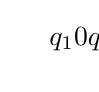
\begin{tikzpicture}[level distance=2cm,sibling distance=.5cm,
   edge from parent path={(\tikzparentnode) -> (\tikzchildnode)}, >=latex]
    \Tree[.$q_1$
      \edge[->]node[auto=right]{$0$}; [.$q_1$
        \edge[->]node[auto=right]{$1$}; [.$q_1$
          \edge[->]node[auto=right]{$0$}; [.$q_1$
            \edge[->]node[auto=right]{$1$}; [.$q_1$
              \edge[->]node[auto=right]{$1$}; [.$q_1$
                \edge[->]node[auto=right]{$0$}; [.\node[red]{$q_1$}; ]
              ]
              \edge[->]node[auto=left]{$1$}; [.$q_2$
                \edge[->]node[auto=right]{$0$}; [.\node[red]{$q_3$}; ]
                \edge[->]node[auto=left]{$\varepsilon$}; [.\node[red]{$q_3$}; ]
              ]
            ]
            \edge[->]node[auto=left]{$1$}; [.$q_2$
              \edge[->]node[auto=right]{$\varepsilon$}; [.$q_3$
                \edge[->]node[auto=right]{$1$}; [.$q_4$
                  \edge[->]node[auto=right]{$0$}; [.\node[blue]{$q_4$}; ]
                ]
              ]
            ]
          ]
        ]
        \edge[->]node[auto=left]{$1$}; [.$q_2$
          \edge[->]node[auto=right]{$0$}; [.$q_3$
            \edge[->]node[auto=right]{$1$}; [.$q_4$
              \edge[->]node[auto=right]{$1$}; [.$q_4$
                \edge[->]node[auto=right]{$0$}; [.\node[blue]{$q_4$}; ]
              ]
            ]
          ]
          \edge[->]node[auto=left]{$\varepsilon$}; [.$q_3$
            \edge[->]node[auto=right]{$0$}; [.$q_4$
              \edge[->]node[auto=right]{$1$}; [.$q_4$
                \edge[->]node[auto=right]{$1$}; [.$q_4$
                  \edge[->]node[auto=right]{$0$}; [.\node[blue]{$q_4$}; ]
                ]
              ]
            ]
          ]
        ]
     ]
   ]
  \end{tikzpicture}
\end{center}

Cada ramo dessa árvore representa uma possível execução do autômato para a entrada dada.
O autômato para apenas quando toda a entrada foi consumida.
Note que nos três ramos mais a esquerda quando isso ocorre não estamos em um estado final, mas nas três da direita sim.
Basta que exita um ramo, uma possibilidade de execução, para que a string seja aceita.
Assim, neste caso a string de fato é aceita, basta escolher um caminha que termine em um estado final.
Por exemplo: $q_1, q_1, q_2, q_2, q_3, q_4, q_4, q_4$ satisfaz a definição para a string $0101\varepsilon 10 = 010110$.

\begin{displaymath}
  L(N_1) = \{\omega \in \{0,1\}^* : \omega \textrm{ contém 101 ou 11 como substring}\}
\end{displaymath}
\end{example}


\begin{example}
    \begin{displaymath}
    N_2 = \langle \{q_1, q_2, q_3, q_4\}, \{0,1\}, \Delta, q_1, \{q_4\}\rangle
  \end{displaymath}

  \begin{center}
  \begin{tabular}{c|ccc}
    $\Delta$ & $0$ & $1$ & $\varepsilon$\\
    \hline
    $q_1$ & $\{q_1\}$ & $\{q_1,q_2\}$ & $\emptyset$\\
    $q_2$ & $\{q_3\}$ & $\{q_3\}$ & $\emptyset$\\
    $q_3$ & $\{q_4\}$ & $\{q_4\}$ & $\emptyset$\\
    $q_4$ & $\emptyset$ & $\emptyset$ & $\emptyset$\\
  \end{tabular}
  \end{center}

  \begin{center}
    \begin{tikzpicture}[node distance=2cm,auto,>=latex,initial text=]
      \tikzset{initial text={}}
      \node[state, initial] (q1) {$q_1$};
      \node[state] (q2) at (3,0) {$q_2$};
      \node[state] (q3) at (6,0) {$q_3$};
      \node[state, accepting] (q4) at (9,0) {$q_4$};
      \path[->] (q1) edge[loop above] node {$0,1$} (q1);
      \path[->] (q1) edge node {$1$} (q2);
      \path[->] (q2) edge node {$0, 1$} (q3);
      \path[->] (q3) edge node {$0, 1$} (q4);
    \end{tikzpicture}
  \end{center}
\begin{displaymath}
  L(N_2) = \{\omega \in \{0,1\}^* : \omega \textrm{ contém 1 na antepenúltima posição}\}
\end{displaymath}
\end{example}

\begin{example}
  A partir daqui vamos apresentar os autômatos apenas por seu diagrama.
  O seguinte é o diagrama de $N_3$:

  \begin{center}
    \begin{tikzpicture}[node distance=2cm,auto,>=latex,initial text=]
      \tikzset{initial text={}}
      \node[state, initial] (q1) {$q_1$};
      \node[state, accepting] (q2) at (2,1) {$q_2$};
      \node[state] (q3) at (6,1) {$q_3$};
      \node[state, accepting] (q4) at (2,-1) {$q_4$};
      \node[state] (q5) at (4,-3) {$q_5$};
      \node[state] (q6) at (6,-1) {$q_6$};
      \path[->] (q1) edge node {$\varepsilon$} (q2);
      \path[->] (q1) edge node {$\varepsilon$} (q4);
      \path[->, bend left = 30] (q2) edge node {$0$} (q3);
      \path[->, bend left = 30] (q3) edge node {$0$} (q2);
      \path[->] (q4) edge node {$0$} (q5);
      \path[->] (q5) edge node {$0$} (q6);
      \path[->] (q6) edge node[above] {$0$} (q4);
    \end{tikzpicture}
  \end{center}
\begin{displaymath}
  L(N_3) = \{\omega \in \{0\}^* : |\omega| \textrm{ é múltiplo de 2 ou de 3}\}
\end{displaymath}
\end{example}

\begin{example}
  O seguinte é o diagrama de $N_4$:

  \begin{center}
    \begin{tikzpicture}[node distance=2cm,auto,>=latex,initial text=]
      \tikzset{initial text={}}
      \node[state, initial] (q1) {$q_1$};
      \node[state, accepting] (q2) at (3,0) {$q_2$};
      \node[state] (q3) at (6,0) {$q_3$};
      \node[state, accepting] (q4) at (9,0) {$q_4$};
      \path[->] (q1) edge[loop above] node {$0,1$} (q1);
      \path[->] (q1) edge node {$0$} (q2);
      \path[->] (q2) edge node {$1$} (q3);
      \path[->] (q3) edge node {$0$} (q4);
    \end{tikzpicture}
  \end{center}
\begin{displaymath}
  L(N_4) = \{\omega \in \{0,1\}^* : |\omega| \textrm{ termina com } 010\}
\end{displaymath}
\end{example}

\begin{example}
  A partir daqui vamos apresentar os autômatos apenas por seu diagrama.
  O seguinte é o diagrama de $N_3$:

  \begin{center}
    \begin{tikzpicture}[node distance=2cm,auto,>=latex,initial text=]
      \tikzset{initial text={}}
      \node[state, initial] (q1) {$q_1$};
      \node[state] (q2) at (2,1.5) {$q_2$};
      \node[state] (q3) at (5,1.5) {$q_3$};
      \node[state] (q4) at (2,-1.5) {$q_4$};
      \node[state, accepting] (q5) at (5,-1.5) {$q_5$};
      \path[->] (q2) edge[loop above] node {$0,1$} (q2);
      \path[->] (q3) edge[loop above] node {$0,1$} (q3);
      \path[->] (q4) edge[loop above] node {$1$} (q4);
      \path[->] (q5) edge[loop above] node {$1$} (q5);
      \path[->] (q1) edge node {$\varepsilon$} (q2);
      \path[->] (q1) edge node {$\varepsilon$} (q4);
      \path[->] (q2) edge node {$1$} (q3);
      \path[->, bend left = 30] (q4) edge node {$0$} (q5);
      \path[->, bend left = 30] (q5) edge node {$0$} (q4);
    \end{tikzpicture}
  \end{center}
\begin{displaymath}
  L(N_5) = \{\omega \in \{0,1\}^* : \omega \textrm{ contém 1 ou um número ímpar de 0s}\}
\end{displaymath}
\end{example}

\begin{example}
  O seguinte é o diagrama de $N_6$:

  \begin{center}
    \begin{tikzpicture}[node distance=2cm,auto,>=latex,initial text=]
      \tikzset{initial text={}}
      \node[state, initial] (q1) {$q_1$};
      \node[state] (q2) at (3,0) {$q_2$};
      \node[state, accepting] (q3) at (6,0) {$q_3$};
      \path[->] (q1) edge[loop above] node {$0$} (q1);
      \path[->] (q2) edge[loop above] node {$1$} (q2);
      \path[->] (q3) edge[loop above] node {$0$} (q3);
      \path[->] (q1) edge node {$1$} (q2);
      \path[->] (q2) edge node {$\varepsilon$} (q3);
    \end{tikzpicture}
  \end{center}
\begin{displaymath}
  L(N_6) = L(0^\star11^\star0^\star)
\end{displaymath}
\end{example}

\section{AFD $\equiv$ AFN}
\label{sec:afn-afd}

Vimos nas últimas seções dois modelos computacionais.
O primeiro é mais próximo da descrição de dispositivos simples, mas sua descrição em termos de diagramas possui diversas limitações.
O segundo modelo é mais flexível e mais fácil de descrever pictoricamente.

A pergunta que procuraremos responder nessa seção é se algum desses modelos é mais expressivo que o outro.
Ou seja, será que algum deles é capaz de resolver problemas, reconhecer linguagens, que o outro não consegue.
A resposta será negativa.
De fato, ambos os modelos são equivalentes em um sentido bastante preciso.
Comecemos então com essa definição.

Dois autômatos $M_1$ e $M_2$ são ditos {\em equivalentes} (escrevemos $M_1 \sim M_2$) se reconhecem a mesma linguagem, ou seja, se $L(M_1) = L(M_2)$.

\medskip
\refstepcounter{theorem}
{\bf Exemplo~\thetheorem:}
%\begin{example}
\begin{multicols}{2}
  \begin{displaymath}
    M_1 = \langle \{q_1, q_2\}, \{a\}, \delta, q_1, \{q_1, q_2\}\rangle
  \end{displaymath}

  \begin{center}
  \begin{tabular}{c|cc}
    $\delta$ & $a$ \\
    \hline
    $q_1$ & $q_2$ \\
    $q_2$ & $q_1$ \\
  \end{tabular}
  \end{center}

  \begin{center}
    \begin{tikzpicture}[node distance=2cm,auto,>=latex,initial text=]
      \tikzset{initial text={}}
      \node[state, initial, accepting] (q1) {$q_1$};
      \node[state, accepting] (q2) at (3,0) {$q_2$};
      \path[->, bend left = 30] (q1) edge node {$a$} (q2);
      \path[->, bend left = 30] (q2) edge node {$a$} (q1);
    \end{tikzpicture}
  \end{center}

  \begin{displaymath}
    L(M_1) = L(a^\star)
  \end{displaymath}

 \columnbreak

  \begin{displaymath}
    M_2 = \langle \{q_1\}, \{a\}, \delta, q_1, \{q_1\}\rangle
  \end{displaymath}

  \begin{center}
  \begin{tabular}{c|cc}
    $\delta$ & $a$ \\
    \hline
    $q_1$ & $q_1$ \\
  \end{tabular}
  \end{center}

  \begin{center}
    \begin{tikzpicture}[node distance=2cm,auto,>=latex,initial text=]
      \tikzset{initial text={}}
      \node[state, initial, accepting] (q1) {$q_1$};
      \path[->] (q1) edge[loop above] node {$a$} (q1);
    \end{tikzpicture}
  \end{center}

  \begin{displaymath}
    L(M_2) = L(a^\star)
  \end{displaymath}
\end{multicols}

  \begin{displaymath}
    M_1 \sim M_2
  \end{displaymath}
%\end{example}
\medskip

Primeiramente devemos mostrar que AFNs são uma extensão dos AFDs.
Essa parte coincide com nossa intuição uma vez que todo diagrama de um AFD é também um diagrama para um AFN (o contrário não vale!).
Vamos formalizar essa ideia no seguinte teorema:


\begin{theorem}
  Se $M$ é um AFD então existe um AFN $N$ tal que $M \sim N$
\end{theorem}
\begin{proof}
  Seja $M = \langle Q, \Sigma, \delta, q_o, F \rangle$ um AFD qualquer.
  Considere o AFN $N = \langle Q, \Sigma, \Delta, q_0, F \rangle$ em que:
\begin{displaymath}
 \Delta(a, q) = \left\{
 \begin{array}{cl}
   \{q'\} & \textrm{se $a \in \Sigma$ e }  \delta(a,q) = q'\\
   \emptyset & \textrm{se } a = \epsilon
 \end{array} \right.
\end{displaymath}

Note que os diagramas de $M$ e de $N$ são idênticos e segue trivialmente que $M \sim N$
\end{proof}

A demonstração da outra equivalência exige mais cuidado e faremos em duas partes.
Primeiro vamos supor que não fosse permitido mudar de estado sem consumir símbolos em um AFN.
Ou seja, suponhamos que não seja permitido usar $\varepsilon$ nas setas no diagrama de estados.
Vamos mostrar que é possível construir um AFD equivalente a esse AFN.
A ideia da construção é que cada estado no AFD simula um conjunto de estados no AFN.
Conforme consumimos a string nesse AFD o estado atual representa o conjunto de todos os estados possíveis no AFN ao consumir os mesmos símbolos.


\begin{lemma}
  Seja $N$ um AFN em que não é permitido mudar de estados sem consumir símbolos, então existe um AFD $M$ tal que $N \sim M$.
\end{lemma}
\begin{proof}
  Não faremos a demonstração completa, apenas apresentaremos a construção e posteriormente mostraremos alguns exemplos.

  Seja $N = \langle Q, \Sigma, \Delta, q_0, F \rangle$, construiremos $M = \langle Q', \Sigma', \delta, q_0', F' \rangle$ da seguinte forma:

  \begin{enumerate}
  \item $Q' = 2^Q$
  \item $\Sigma' = \Sigma$
  \item $q_0' = \{q_0 \}$
  \item $F' = \{R \in Q' : R \cap F \neq \emptyset\}$
  \item $\delta(R, a) = \bigcup_{r \in R} \Delta(r,a)$
  \end{enumerate}
\end{proof}

\begin{example}
\begin{displaymath}
  N_1 = \langle \{1,2\}, \{a,b\}, \Delta, 1, \{1\}\rangle
\end{displaymath}
\begin{center}
  \begin{tabular}{c|cc}
    $\Delta$ & $a$         & $b$\\
    \hline
    $1$      & $\emptyset$ & $\{2\}$\\
    $2$      & $\{1,2\}$   & $\{1\}$\\
  \end{tabular}
\end{center}

  \begin{center}
    \begin{tikzpicture}[node distance=2cm,auto,>=latex,initial text=]
      \tikzset{initial text={}}
      \node[state, initial, accepting] (1) {$1$};
      \node[state] (2) at (3,0) {$2$};
      \path[->, bend left = 30] (1) edge node {$b$} (2);
      \path[->, bend left = 30] (2) edge node {$a,b$} (1);
      \path[->] (2) edge[loop above] node {$a$} (1);
    \end{tikzpicture}
  \end{center}

Seguindo a construção que vimos no teorema anterior:

\begin{displaymath}
  M_1 = \langle \{\emptyset, \{1\}, \{2\}, \{1,2\}\}, \{a,b\}, \delta, \{1\}, \{\{1\}, \{1,2\}\}\rangle
\end{displaymath}
\begin{center}
  \begin{tabular}{c|cc}
    $\delta$     & $a$         & $b$\\
    \hline
    $\emptyset$  & $\emptyset$ & $\emptyset$ \\
    $\{1\}$      & $\emptyset$ & $\{2\}$\\
    $\{2\}$      & $\{1,2\}$   & $\{1\}$\\
    $\{1,2\}$    & $\{1,2\}$   & $\{1,2\}$\\
  \end{tabular}
\end{center}

  \begin{center}
    \begin{tikzpicture}[node distance=2cm,auto,>=latex,initial text=]
      \tikzset{initial text={}}
      \node[state, initial, accepting] (1) {$\{1\}$};
      \node[state] (2) at (3,0) {$\{2\}$};
      \node[state, accepting] (12) at (3, -2){$\{1, 2\}$};
      \node[state] (0) at (0, -2){$\emptyset$};
      \path[->] (1) edge node {$a$} (0);
      \path[->, bend left = 30] (1) edge node {$b$} (2);
      \path[->] (2) edge node {$a$} (12);
      \path[->, bend left = 30] (2) edge node {$b$} (1);
      \path[->] (0) edge[loop below] node {$a,b$} (0);
      \path[->] (12) edge[loop below] node {$a,b$} (12);
    \end{tikzpicture}
  \end{center}

Para terminar vamos simular nos dois a leitura da string $baab$:

\begin{multicols}{2}

\begin{center}
  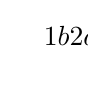
\begin{tikzpicture}[level distance=2cm,sibling distance=.5cm,
   edge from parent path={(\tikzparentnode) -> (\tikzchildnode)}, >=latex]
    \Tree[.$1$
      \edge[->]node[auto=right]{$b$}; [.$2$
        \edge[->]node[auto=right]{$a$}; [.\node[red]{$1$}; ]
        \edge[->]node[auto=left]{$a$}; [.$2$
          \edge[->]node[auto=right]{$a$}; [.$1$
            \edge[->]node[auto=right]{$b$}; [.\node[red]{$2$}; ]
          ]
          \edge[->]node[auto=left]{$a$}; [.$2$
            \edge[->]node[auto=left]{$b$}; [.\node[blue]{$1$}; ]
          ]
        ]
      ]
    ]
  \end{tikzpicture}
\end{center}
\columnbreak

\begin{center}
  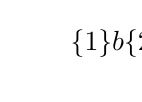
\begin{tikzpicture}[level distance=2cm,sibling distance=.5cm,
   edge from parent path={(\tikzparentnode) -> (\tikzchildnode)}, >=latex]
    \Tree[.$\{1\}$
      \edge[->]node[auto=right]{$b$}; [.$\{2\}$
        \edge[->]node[auto=right]{$a$}; [.$\{1,2\}$
          \edge[->]node[auto=right]{$a$}; [.$\{1,2\}$
            \edge[->]node[auto=right]{$b$}; [.\node[blue]{$\{1,2\}$}; ]
          ]
        ]
      ]
    ]
  \end{tikzpicture}
\end{center}
\end{multicols}
\end{example}

Para completar nossa prova precisamos lidar com as setas rotuladas por $\varepsilon$.
O que faremos nesse caso incluir no estado atual todos os estados que conseguimos alcançar sem precisar consumir símbolos.


\begin{theorem}
  Para todo AFN $N$ existe um AFD $M$ tal que $N \sim M$.
\end{theorem}
\begin{proof}
  Sejam $N$ e $M$ como definidos na demonstração do lema anterior
  Considere a seguinte função $E: Q' \to Q'$:
  \begin{displaymath}
    E(R) = \{q \in Q: \exists q' \in R(q' \stackrel{\varepsilon}{\rightsquigarrow} q) \}
  \end{displaymath}
  Ou seja, existe um caminho de algum $q' \in R$ até $q$ passando apenas por setas com etiqueta $\varepsilon$.

  Vamos agora atualizar a definição de $M$ em dois pontos:

  \begin{enumerate}
  \item[3'.] $q_0 = E(\{q_0\})$
  \item[5'.] $\delta(R,a) = \bigcup_{r \in R} E(\Delta(r,a))$
  \end{enumerate}
\end{proof}


\begin{example}
  Considere o AFN $N_2$ representado pelo seguinte diagrama de estados:

  \begin{center}
    \begin{tikzpicture}[node distance=2cm,auto,>=latex,initial text=]
      \tikzset{initial text={}}
      \node[state, initial] (q1) {$q_1$};
      \node[state] (q2) at (3,0) {$q_2$};
      \node[state, accepting] (q3) at (6,0){$q_3$};
      \path[->] (q1) edge node {$1$} (q2);
      \path[->] (q2) edge node {$\varepsilon$} (q3);
      \path[->] (q1) edge[loop above] node {$0$} (q1);
      \path[->] (q2) edge[loop above] node {$1$} (q2);
      \path[->] (q3) edge[loop above] node {$0$} (q3);
    \end{tikzpicture}
  \end{center}

  \begin{displaymath}
    L(N_2) = L(0^\star11^\star0^\star)
  \end{displaymath}

  Usando a construção dos teoremas anteriores produzimos o seguinte AFD $M_2$:

  \begin{center}
    \begin{tikzpicture}[node distance=2cm,auto,>=latex,initial text=]
      \tikzset{initial text={}}
      \node[state, initial] (1) {$\{q_1\}$};
      \node[state, accepting] (23) at (3,0) {$\{q_2,q_3\}$};
      \node[state, accepting, red] (123) at (6,0){$Q$};
      \node[state, red] (2) at (0,3) {$\{q_2\}$};
      \node[state] (0) at (3,3) {$\{\emptyset\}$};
      \node[state, accepting] (3) at (6,3){$\{q_3\}$};
      \node[state, red] (12) at (1,-3) {$\{q_1, q_2\}$};
      \node[state, accepting, red] (13) at (5,-3){$\{q_1,q_3\}$};
      \path[->] (0) edge[loop above] node {$0,1$} (0);
      \path[->] (1) edge[loop above] node {$0$} (1);
      \path[->] (1) edge node {$1$} (23);
      \path[->] (2) edge node {$0$} (0);
      \path[->] (2) edge node {$1$} (23);
      \path[->] (3) edge[loop above] node {$0$} (3);
      \path[->] (3) edge node {$1$} (0);
      \path[->] (12) edge node {$0$} (1);
      \path[->] (12) edge node {$1$} (23);
      \path[->] (13) edge[loop below] node {$0$} (13);
      \path[->] (13) edge node {$1$} (23);
      \path[->] (23) edge node {$0$} (3);
      \path[->] (23) edge[loop above] node {$1$} (23);
      \path[->] (123) edge node {$0$} (13);
      \path[->] (123) edge node {$1$} (23);
    \end{tikzpicture}
  \end{center}

A construção que vimos possui sempre uma quantidade exponencialmente maior de estados, porém, alguns deles podem ser supérfluos.
Note que os estados em vermelho não são alcançáveis a partir do estado inicial, logo, podem ser omitidos (formalmente, o autômato gerado ao se omitir esses estados é equivalente a esse).

 \begin{center}
    \begin{tikzpicture}[node distance=2cm,auto,>=latex,initial text=]
      \tikzset{initial text={}}
      \node[state, initial] (1) {$\{q_1\}$};
      \node[state, accepting] (23) at (3,0) {$\{q_2,q_3\}$};
      \node[state, accepting] (3) at (6,0){$\{q_3\}$};
      \node[state] (0) at (9,0){$\emptyset$};
      \path[->] (1) edge node {$1$} (23);
      \path[->] (23) edge node {$0$} (3);
      \path[->] (3) edge node {$1$} (0);
      \path[->] (1) edge[loop above] node {$0$} (1);
      \path[->] (23) edge[loop above] node {$1$} (23);
      \path[->] (3) edge[loop above] node {$0$} (3);
      \path[->] (0) edge[loop above] node {$0,1$} (0);
    \end{tikzpicture}
  \end{center}

  Removendo os estados supérfluos é fácil ver que:
  \begin{displaymath}
    L(M_2) = L(N_2) = L(0^\star11^\star0^\star)
  \end{displaymath}
  Portanto $M_2 \sim N_2$.
\end{example}


\section{Linguagens Regulares são Reconhecíveis por AFNs}
\label{sec:rg-afn}

Na seção anterior vimos que AFDs e AFNs são capazes de reconhecer a mesma classe de linguagens.
Nesta seção começaremos a investigar que essa classe é exatamente a classe das linguagens regulares.

Mostraremos nessa seção que toda linguagem regular é reconhecível por algum AFN e, consequentemente, por algum AFD.
Para tanto, temos que mostrar que a classe das linguagens reconhecíveis por AFNs é fechada por $*$, $\cup$, $\circ$ e que contém $\{\{a\} : a \in \Sigma\}$.


\begin{lemma}
  Se $A, B \subseteq \Sigma^*$ são reconhecíveis por AFNs então $A \cup B$ também é.
  Ou seja, a classe das linguagens reconhecíveis por AFNs é fechada por união.
\end{lemma}
\begin{proof}
  A hipótese garante que existem AFNs $N_1$ e $N_2$ tal que $L(N_1) = A$ e $L(N_2) = B$.
  Vamos construir a partir de $N_1$ e $N_2$ um AFN $N$ tal que $L(N) = L(N_1) \cup L(N_2)$

  Sejam:

  \begin{eqnarray*}
    N_1 & = & \langle Q_1, \Sigma, \Delta_1, q_1, F_1 \rangle\\
    N_2 & = & \langle Q_2, \Sigma, \Delta_2, q_1, F_2 \rangle
  \end{eqnarray*}

  Vamos construir $N = \langle Q, \Sigma, \Delta, q_0, F \rangle$:

  \begin{itemize}
  \item[] $Q = Q_1 \cup Q_2 \cup \{q_0\}$
  \item[] $F = F_1 \cup F_2$
  \item[] $\Delta(q,a) = \left\{
    \begin{array}{ccc}
      \Delta_1(q, a) & \textrm{ se } & q \in Q_1\\
      \Delta_2(q, a) & \textrm{ se } & q \in Q_2\\
      \{q_1, q_2\}   & \textrm{ se } & q = q_0 \textrm{ e } a = \varepsilon \\
      \emptyset     & \textrm{ se }  & q = q_0 \textrm{ e } a \neq \varepsilon \\
    \end{array}\right.$
  \end{itemize}

  \begin{multicols}{2}
   $N_1$
 \begin{center}
    \begin{tikzpicture}[node distance=2cm,auto,>=latex,initial text=,color=blue]
      \tikzset{
        coil/.style={ decorate, decoration={ snake=coil} },
      }
      \node[state, initial] (1) {$q_1$};
      \node[state, accepting, minimum size=0pt] (2) at (3,1){};
      \node[state, accepting, minimum size=0pt] (3) at (3,0){};
      \node[state, accepting, minimum size=0pt] (4) at (3,-1){};
      \path[->] (1) edge[coil]  (2);
      \path[->] (1) edge[coil]  (3);
      \path[->] (1) edge[coil]  (4);
    \end{tikzpicture}
  \end{center}
    \columnbreak
    $N_2$
    \begin{center}
    \begin{tikzpicture}[node distance=2cm,auto,>=latex,initial text=,color=red]
      \tikzset{
        coil/.style={ decorate, decoration={ snake=coil} },
      }
      \node[state, initial] (1) {$q_2$};
      \node[state, accepting, minimum size=0pt] (2) at (3,1){};
      \node[state, accepting, minimum size=0pt] (4) at (3,-1){};
      \path[->] (1) edge[coil]  (2);
      \path[->] (1) edge[coil]  (4);
    \end{tikzpicture}
  \end{center}
  \end{multicols}
    $N$
    \begin{center}
    \begin{tikzpicture}[node distance=2cm,auto,>=latex,initial text=]
      \tikzset{
        coil/.style={ decorate, decoration={ snake=coil} },
      }
      \node[state, initial] (0) {$q_0$};
      \node[state, color=blue] (1) at (2,1) {$q_1$};
      \node[state, color=red] (2) at (2,-1) {$q_2$};
      \node[state, accepting, minimum size=0pt, color=blue] (f1) at (5,2){};
      \node[state, accepting, minimum size=0pt, color=blue] (f2) at (5,1){};
      \node[state, accepting, minimum size=0pt, color=blue] (f3) at (5,0){};
      \node[state, accepting, minimum size=0pt, color=red] (f4) at (5,-1){};
      \node[state, accepting, minimum size=0pt, color=red] (f5) at (5,-2){};
      \path[->] (0) edge node {$\varepsilon$} (1);
      \path[->] (0) edge node {$\varepsilon$} (2);
      \path[->, color=blue] (1) edge[coil]  (f1);
      \path[->, color=blue] (1) edge[coil]  (f2);
      \path[->, color=blue] (1) edge[coil]  (f3);
      \path[->, color=red] (2) edge[coil]  (f4);
      \path[->, color=red] (2) edge[coil]  (f5);
    \end{tikzpicture}
  \end{center}
\end{proof}


\begin{example}
  \begin{multicols}{2}
   $N_1$
 \begin{center}
    \begin{tikzpicture}[node distance=2cm,auto,>=latex,initial text=]
      \node[state, initial, accepting] (1) {$q_1$};
      \path[->] (1) edge[loop above] node {$0$} (1);
    \end{tikzpicture}
  \end{center}
  \begin{displaymath}
    L(N_1) = L(0^\star)
  \end{displaymath}

    \columnbreak
    $N_2$
    \begin{center}
    \begin{tikzpicture}[node distance=2cm,auto,>=latex,initial text=]
      \node[state, initial] (2) {$q_2$};
      \node[state, accepting] (3) at (3,0){$q_3$};
      \path[->] (3) edge[loop above] node {$0$} (3);
      \path[->] (2) edge node{$1$}  (3);
    \end{tikzpicture}
  \end{center}
  \begin{displaymath}
    L(N_2) = L(10^\star)
  \end{displaymath}

  \end{multicols}
    $N$
    \begin{center}
    \begin{tikzpicture}[node distance=2cm,auto,>=latex,initial text=]
      \node[state, initial] (0) {$q_0$};
      \node[state, accepting] (1) at (2, 1){$q_1$};
      \node[state] (2) at (2, -1){$q_2$};
      \node[state, accepting] (3) at (5, -1){$q_3$};
      \path[->] (1) edge[loop above] node {$0$} (1);
      \path[->] (3) edge[loop above] node {$0$} (3);
      \path[->] (2) edge node{$1$}  (3);
      \path[->] (0) edge node{$\varepsilon$}  (1);
      \path[->] (0) edge node{$\varepsilon$}  (2);
    \end{tikzpicture}
  \end{center}
\begin{displaymath}
  L(N) = L(N_1) \cup L(N_2) = L(0^\star) \cup L(10^\star) = L(0^\star \abxcup 10^\star)
\end{displaymath}

\end{example}


\begin{lemma}
Se $A, B \subseteq \Sigma^*$ são reconhecíveis por AFNs então $A \circ B$ também é.
  Ou seja, a classe das linguagens reconhecíveis por AFNs é fechada por concatenação.
\end{lemma}
\begin{proof}
  A hipótese garante que existem AFNs $N_1$ e $N_2$ tal que $L(N_1) = A$ e $L(N_2) = B$.
  Vamos construir a partir de $N_1$ e $N_2$ um AFN $N$ tal que $L(N) = L(N_1) \circ L(N_2)$

  Sejam:

  \begin{eqnarray*}
    N_1 & = & \langle Q_1, \Sigma, \Delta_1, q_1, F_1 \rangle\\
    N_2 & = & \langle Q_2, \Sigma, \Delta_2, q_1, F_2 \rangle
  \end{eqnarray*}

  Vamos construir $N = \langle Q, \Sigma, \Delta, q_0, F \rangle$:

  \begin{itemize}
  \item[] $Q = Q_1 \cup Q_2$
  \item[] $q_0 = q_1$
  \item[] $F = F_2$
  \item[] $\Delta(q,a) = \left\{
    \begin{array}{ccc}
      \Delta_1(q, a) & \textrm{ se } & q \in Q_1 \textrm{ e } q \notin F_1\\
      \Delta_1(q, a) & \textrm{ se } & q \in F_1 \textrm{ e } a \neq \varepsilon\\
      \Delta_1(q, a) \cup \{q_2\} & \textrm{ se } & q \in F_1 \textrm{ e } a = \varepsilon\\
      \Delta_2(q, a) & \textrm{ se } & q \in Q_2\\
     \end{array}\right.$
  \end{itemize}

  \begin{multicols}{2}
   $N_1$
 \begin{center}
    \begin{tikzpicture}[node distance=2cm,auto,>=latex,initial text=,color=blue]
      \tikzset{
        coil/.style={ decorate, decoration={ snake=coil} },
      }
      \node[state, initial] (1) {$q_1$};
      \node[state, accepting, minimum size=0pt] (2) at (3,1){};
      \node[state, accepting, minimum size=0pt] (3) at (3,0){};
      \node[state, accepting, minimum size=0pt] (4) at (3,-1){};
      \path[->] (1) edge[coil]  (2);
      \path[->] (1) edge[coil]  (3);
      \path[->] (1) edge[coil]  (4);
    \end{tikzpicture}
  \end{center}
    \columnbreak
    $N_2$
    \begin{center}
    \begin{tikzpicture}[node distance=2cm,auto,>=latex,initial text=,color=red]
      \tikzset{
        coil/.style={ decorate, decoration={ snake=coil} },
      }
      \node[state, initial] (1) {$q_2$};
      \node[state, accepting, minimum size=0pt] (2) at (3,1){};
      \node[state, accepting, minimum size=0pt] (4) at (3,-1){};
      \path[->] (1) edge[coil]  (2);
      \path[->] (1) edge[coil]  (4);
    \end{tikzpicture}
  \end{center}
  \end{multicols}
    $N$
    \begin{center}
    \begin{tikzpicture}[node distance=2cm,auto,>=latex,initial text=]
      \tikzset{
        coil/.style={ decorate, decoration={ snake=coil} },
      }
      \node[state, initial, color=blue] (1) {$q_1$};
      \node[state, minimum size=0pt, color=blue] (f1) at (3,1){};
      \node[state, minimum size=0pt, color=blue] (f2) at (3,0){};
      \node[state, minimum size=0pt, color=blue] (f3) at (3,-1){};
      \node[state, color=red] (2) at (5,0) {$q_2$};
      \node[state, accepting, minimum size=0pt, color=red] (f4) at (8,1){};
      \node[state, accepting, minimum size=0pt, color=red] (f5) at (8,-1){};
      \path[->] (f1) edge node {$\varepsilon$} (2);
      \path[->] (f2) edge node {$\varepsilon$} (2);
      \path[->] (f3) edge node {$\varepsilon$} (2);
      \path[->, color=blue] (1) edge[coil]  (f1);
      \path[->, color=blue] (1) edge[coil]  (f2);
      \path[->, color=blue] (1) edge[coil]  (f3);
      \path[->, color=red] (2) edge[coil]  (f4);
      \path[->, color=red] (2) edge[coil]  (f5);
    \end{tikzpicture}
  \end{center}
\end{proof}


\begin{example}
  \begin{multicols}{2}
   $N_1$
 \begin{center}
    \begin{tikzpicture}[node distance=2cm,auto,>=latex,initial text=]
      \node[state, initial, accepting] (1) {$q_1$};
      \path[->] (1) edge[loop above] node {$0$} (1);
    \end{tikzpicture}
  \end{center}
  \begin{displaymath}
    L(N_1) = L(0^\star)
  \end{displaymath}

    \columnbreak
    $N_2$
    \begin{center}
    \begin{tikzpicture}[node distance=2cm,auto,>=latex,initial text=]
      \node[state, initial] (2) {$q_2$};
      \node[state, accepting] (3) at (3,0){$q_3$};
      \path[->] (3) edge[loop above] node {$0$} (3);
      \path[->] (2) edge node{$1$}  (3);
    \end{tikzpicture}
  \end{center}
  \begin{displaymath}
    L(N_2) = L(10^\star)
  \end{displaymath}

  \end{multicols}
    $N$
    \begin{center}
    \begin{tikzpicture}[node distance=2cm,auto,>=latex,initial text=]
      \node[state, initial] (1) {$q_1$};
      \node[state] (2) at (3, 0){$q_2$};
      \node[state, accepting] (3) at (6, 0){$q_3$};
      \path[->] (1) edge[loop above] node {$0$} (1);
      \path[->] (3) edge[loop above] node {$0$} (3);
      \path[->] (2) edge node{$1$}  (3);
      \path[->] (1) edge node{$\varepsilon$}  (2);
    \end{tikzpicture}
  \end{center}
\begin{displaymath}
  L(N) = L(N_1) \circ L(N_2) = L(0^\star) \circ L(10^\star) = L(0^\star 10^\star)
\end{displaymath}

\end{example}

\begin{lemma}
  Se $A \subseteq \Sigma^*$ é reconhecível por um AFN então $A^*$ também é.
  Ou seja, a classe das linguagens reconhecíveis por AFNs é fechada por estrela de Kleene.
\end{lemma}
\begin{proof}
  A hipótese garante que existe AFNs $N_1$ tal que $L(N_1) = A$.
  Vamos construir a partir de $N_1$ um AFN $N$ tal que $L(N) = L(N_1)^*$

  Seja:

  \begin{eqnarray*}
    N_1 & = & \langle Q_1, \Sigma, \Delta_1, q_1, F_1 \rangle\\
  \end{eqnarray*}

  Vamos construir $N = \langle Q, \Sigma, \Delta, q_0, F \rangle$:

  \begin{itemize}
  \item[] $Q = Q_1 \cup \{q_0\}$
  \item[] $F = F_1 \cup \{q_0\}$
  \item[] $\Delta(q,a) = \left\{
    \begin{array}{ccc}
      \Delta_1(q, a) & \textrm{ se } & q \in Q_1 \textrm{ e } q \notin F_1\\
      \Delta_1(q, a) & \textrm{ se } & q \in F_1 \textrm{ e } a \neq \varepsilon\\
      \Delta_1(q, a) \cup \{q_1\} & \textrm{ se } & q \in F_1 \textrm{ e } a = \varepsilon\\
      \{q_1\} & \textrm{ se } & q = q_0 \textrm{ e } a = \varepsilon\\
      \emptyset & \textrm{ se } & q = q_0 \textrm{ e } a \neq \varepsilon\\
     \end{array}\right.$
  \end{itemize}

   $N_1$
 \begin{center}
    \begin{tikzpicture}[node distance=2cm,auto,>=latex,initial text=,color=blue]
      \tikzset{
        coil/.style={ decorate, decoration={ snake=coil} },
      }
      \node[state, initial] (1) {$q_1$};
      \node[state, accepting, minimum size=0pt] (2) at (3,1){};
      \node[state, accepting, minimum size=0pt] (3) at (3,0){};
      \node[state, accepting, minimum size=0pt] (4) at (3,-1){};
      \path[->] (1) edge[coil]  (2);
      \path[->] (1) edge[coil]  (3);
      \path[->] (1) edge[coil]  (4);
    \end{tikzpicture}
  \end{center}

    $N$
    \begin{center}
    \begin{tikzpicture}[node distance=2cm,auto,>=latex,initial text=]
      \tikzset{
        coil/.style={ decorate, decoration={ snake=coil} },
      }
      \node[state, initial, accepting] (0) {$q_0$};
      \node[state, color=blue] (1) at (2,0) {$q_1$};
      \node[state, accepting, minimum size=0pt, color=blue] (f1) at (5,2){};
      \node[state, accepting, minimum size=0pt, color=blue] (f2) at (5,0){};
      \node[state, accepting, minimum size=0pt, color=blue] (f3) at (5,-2){};
      \path[->] (0) edge node {$\varepsilon$} (1);
      \path[->, color=blue] (1) edge[coil]  (f1);
      \path[->, color=blue] (1) edge[coil]  (f2);
      \path[->, color=blue] (1) edge[coil]  (f3);
      \path[->, bend right = 30] (f1) edge node[above]{$\varepsilon$}  (1);
      \path[->, bend right = 30] (f2) edge node[above]{$\varepsilon$}  (1);
      \path[->, bend left = 30] (f3) edge node {$\varepsilon$}  (1);
    \end{tikzpicture}
  \end{center}
\end{proof}


\begin{example}

   $N_1$
   \begin{center}
    \begin{tikzpicture}[node distance=2cm,auto,>=latex,initial text=]
      \node[state, initial] (1) {$q_1$};
      \node[state] (2) at (3,1){$q_2$};
      \node[state, accepting] (3) at (6,1){$q_3$};
      \node[state] (4) at (3,-1){$q_4$};
      \node[state, accepting] (5) at (6,-1){$q_5$};
      \path[->] (1) edge node{$0$}  (2);
      \path[->] (1) edge node{$1$}  (4);
      \path[->] (2) edge node{$1$}  (3);
      \path[->] (4) edge node{$0$}  (5);
    \end{tikzpicture}
  \end{center}
  \begin{displaymath}
    L(N_1) = L(01 \abxcup 10)
  \end{displaymath}


    $N$
    \begin{center}
    \begin{tikzpicture}[node distance=2cm,auto,>=latex,initial text=]
      \node[state,initial, accepting] (1) {$q_1$};
      \node[state] (1) at (3,0) {$q_1$};
      \node[state] (2) at (6,1){$q_2$};
      \node[state, accepting] (3) at (9,1){$q_3$};
      \node[state] (4) at (6,-1){$q_4$};
      \node[state, accepting] (5) at (9,-1){$q_5$};
      \path[->] (0) edge node{$\varepsilon$}  (1);
      \path[->] (1) edge node{$0$}  (2);
      \path[->] (1) edge node{$1$}  (4);
      \path[->] (2) edge node{$1$}  (3);
      \path[->] (4) edge node{$0$}  (5);
      \path[->, bend right = 45] (3) edge node[above]{$\varepsilon$}  (1);
      \path[->, bend left = 45] (5) edge node {$\varepsilon$}  (1);
    \end{tikzpicture}
  \end{center}
\begin{displaymath}
  L(N) = L(N_1)^* = L((01 \abxcup 10)^\star)
\end{displaymath}

\end{example}


\begin{theorem}
  Toda linguagem regular é reconhecível por um AFN.
  Ou seja, a classe das linguagens reconhecíveis por AFNs contém a classe das linguagem regulares.
\end{theorem}

\begin{proof}
  Pelos lemas anteriores sabemos que a classe das linguagens reconhecíveis por AFNs é fechada por união, concatenação e estrela de Kleene.
  Para completar a prova mostraremos que a classe contém as linguagens $\{a\}$ para todo $a \in \Sigma$, $\{epsilon\}$ e $\emptyset$.
Os seguintes AFNs fazem exatamente isso:

$N_a$

\begin{center}
  \begin{tikzpicture}[node distance=2cm,auto,>=latex,initial text=]
    \node[state,initial] (1) {$q_1$};
    \node[state, accepting] (2) at (3,0) {$q_2$};
    \path[->] (1) edge node{$a$}  (2);
  \end{tikzpicture}
\end{center}

$N_\varepsilon$
\begin{center}
  \begin{tikzpicture}[node distance=2cm,auto,>=latex,initial text=]
    \node[state,initial,accepting] (1) {$q_1$};
  \end{tikzpicture}
\end{center}

$N_\emptyset$
\begin{center}
  \begin{tikzpicture}[node distance=2cm,auto,>=latex,initial text=]
    \node[state,initial] (1) {$q_1$};
  \end{tikzpicture}
\end{center}
\end{proof}


\begin{example}
  Construiremos o autômato que reconhece $L((ab \abxcup a)^\star)$ usando o método visto neste capítulo:

  $a$
\begin{center}
  \begin{tikzpicture}[node distance=2cm,auto,>=latex,initial text=]
    \node[state, initial, minimum size=0pt] (1) {};
    \node[state, accepting, minimum size=0pt] (2) at (2,0) {};
    \path[->] (1) edge node{$a$}  (2);
  \end{tikzpicture}
\end{center}

  $b$
\begin{center}
  \begin{tikzpicture}[node distance=2cm,auto,>=latex,initial text=]
    \node[state, initial, minimum size=0pt] (1) {};
    \node[state, accepting, minimum size=0pt] (2) at (2,0) {};
    \path[->] (1) edge node{$b$}  (2);
  \end{tikzpicture}
\end{center}

$ab$

\begin{center}
  \begin{tikzpicture}[node distance=2cm,auto,>=latex,initial text=]
    \node[state,initial, minimum size=0pt] (1) {};
    \node[state, minimum size=0pt] (2) at (2,0) {};
    \node[state, minimum size=0pt] (3) at (3,0) {};
    \node[state, accepting, minimum size=0pt] (4) at (5,0) {};
    \path[->] (1) edge node{$a$}  (2);
    \path[->] (2) edge node{$\varepsilon$}  (3);
    \path[->] (3) edge node{$b$}  (4);
  \end{tikzpicture}
\end{center}

$ab \abxcup a$

\begin{center}
  \begin{tikzpicture}[node distance=2cm,auto,>=latex,initial text=]
    \node[state, initial, minimum size=0pt] (1) {};
    \node[state, minimum size=0pt] (2) at (1,0) {};
    \node[state, minimum size=0pt] (3) at (3,0) {};
    \node[state, minimum size=0pt] (4) at (4,0) {};
    \node[state, accepting,minimum size=0pt] (5) at (7,0) {};
    \node[state, minimum size=0pt] (6) at (1,-1){};
    \node[state, accepting, minimum size=0pt] (7) at (3,-1) {};
    \path[->] (1) edge node{$\varepsilon$}  (2);
    \path[->] (1) edge node[below]{$\varepsilon$}  (6);
    \path[->] (2) edge node{$a$}  (3);
    \path[->] (3) edge node{$\varepsilon$}  (4);
    \path[->] (4) edge node{$b$}  (5);
    \path[->] (6) edge node{$a$}  (7);
  \end{tikzpicture}
\end{center}

$(ab \abxcup a)^\star$
\begin{center}
  \begin{tikzpicture}[node distance=2cm,auto,>=latex,initial text=]
    \node[state, initial, accepting, minimum size=0pt] (1) {};
    \node[state, minimum size=0pt] (2) at (1,0) {};
    \node[state, minimum size=0pt] (3) at (2,0) {};
    \node[state, minimum size=0pt] (4) at (4,0) {};
    \node[state, minimum size=0pt] (5) at (5,0) {};
    \node[state, accepting,minimum size=0pt] (6) at (7,0) {};
    \node[state, minimum size=0pt] (7) at (2,-1){};
    \node[state, accepting, minimum size=0pt] (8) at (5,-1) {};
    \path[->] (1) edge node{$\varepsilon$}  (2);
    \path[->] (2) edge node{$\varepsilon$}  (3);
    \path[->] (2) edge node{$\varepsilon$}  (7);
    \path[->] (3) edge node{$a$}  (4);
    \path[->] (4) edge node{$\varepsilon$}  (5);
    \path[->] (5) edge node{$b$}  (6);
    \path[->] (7) edge node{$a$}  (8);
    \path[->, bend left = 60] (8) edge node{$\varepsilon$}  (2);
    \path[->, bend right = 45] (6) edge node[above]{$\varepsilon$}  (2);
  \end{tikzpicture}
\end{center}

\end{example}


\begin{example}
    Para concluir, construiremos o autômato que reconhece $L((a \abxcup b)^\star aba)$ usando o método visto neste capítulo:

$a \abxcup b$

\begin{center}
  \begin{tikzpicture}[node distance=2cm,auto,>=latex,initial text=]
    \node[state, initial, minimum size=0pt] (1) {};
    \node[state, minimum size=0pt] (2) at (1,1) {};
    \node[state, accepting, minimum size=0pt] (3) at (3,1) {};
    \node[state, minimum size=0pt] (6) at (1,-1){};
    \node[state, accepting, minimum size=0pt] (7) at (3,-1) {};
    \path[->] (1) edge node{$\varepsilon$}  (2);
    \path[->] (1) edge node{$\varepsilon$}  (6);
    \path[->] (2) edge node{$a$}  (3);
    \path[->] (6) edge node{$b$}  (7);
  \end{tikzpicture}
\end{center}

$(a \abxcup b)^\star$

\begin{center}
  \begin{tikzpicture}[node distance=2cm,auto,>=latex,initial text=]
    \node[state, initial, accepting, minimum size=0pt] (1) {};
    \node[state, minimum size=0pt] (2) at (1,0){};
    \node[state, minimum size=0pt] (3) at (2,1) {};
    \node[state, accepting, minimum size=0pt] (4) at (4,1) {};
    \node[state, minimum size=0pt] (7) at (2,-1){};
    \node[state, accepting, minimum size=0pt] (8) at (4,-1) {};
    \path[->] (1) edge node{$\varepsilon$}  (2);
    \path[->] (2) edge node[below]{$\varepsilon$}  (3);
    \path[->] (2) edge node{$\varepsilon$}  (7);
    \path[->] (3) edge node{$a$}  (4);
    \path[->] (7) edge node{$b$}  (8);
    \path[->, bend right = 60] (4) edge node[above]{$\varepsilon$}  (2);
    \path[->, bend left = 60] (8) edge node{$\varepsilon$}  (2);
  \end{tikzpicture}
\end{center}

$aba$

\begin{center}
  \begin{tikzpicture}[node distance=2cm,auto,>=latex,initial text=]
    \node[state,initial, minimum size=0pt] (1) {};
    \node[state, minimum size=0pt] (2) at (2,0) {};
    \node[state, minimum size=0pt] (3) at (3,0) {};
    \node[state, minimum size=0pt] (4) at (5,0) {};
    \node[state, minimum size=0pt] (5) at (6,0) {};
    \node[state, accepting, minimum size=0pt] (6) at (8,0) {};
    \path[->] (1) edge node{$a$}  (2);
    \path[->] (2) edge node{$\varepsilon$}  (3);
    \path[->] (3) edge node{$b$}  (4);
    \path[->] (4) edge node{$\varepsilon$}  (5);
    \path[->] (5) edge node{$a$}  (6);
  \end{tikzpicture}
\end{center}



$(a \abxcup b)^\star aba$
\begin{center}
  \begin{tikzpicture}[node distance=2cm,auto,>=latex,initial text=]
    \node[state, initial, minimum size=0pt] (1) {};
    \node[state, minimum size=0pt] (2) at (1,0){};
    \node[state, minimum size=0pt] (3) at (2,1) {};
    \node[state, minimum size=0pt] (4) at (4,1) {};
    \node[state, minimum size=0pt] (5) at (2,-1){};
    \node[state, minimum size=0pt] (6) at (4,-1) {};

    \node[state, minimum size=0pt] (7) at (5,-3){};
    \node[state, minimum size=0pt] (8) at (6,-3) {};
    \node[state, minimum size=0pt] (9) at (7,-3) {};
    \node[state, minimum size=0pt] (10) at (8,-3) {};
    \node[state, minimum size=0pt] (11) at (9,-3) {};
    \node[state, accepting, minimum size=0pt] (12) at (10,-3) {};

    \path[->] (1) edge node{$\varepsilon$}  (2);
    \path[->] (2) edge node[below]{$\varepsilon$}  (3);
    \path[->] (2) edge node{$\varepsilon$}  (5);
    \path[->] (3) edge node{$a$}  (4);
    \path[->] (5) edge node{$b$}  (6);
    \path[->, bend right = 60] (4) edge node[above]{$\varepsilon$}  (2);
    \path[->, bend left = 60] (6) edge node{$\varepsilon$}  (2);

    \path[->] (7) edge node{$a$}  (8);
    \path[->] (8) edge node{$\varepsilon$}  (9);
    \path[->] (9) edge node{$b$}  (10);
    \path[->] (10) edge node{$\varepsilon$}  (11);
    \path[->] (11) edge node{$a$}  (12);

    \path[->, bend right = 45] (1) edge node[below]{$\varepsilon$}  (7);
    \path[->, bend left = 30] (4) edge node{$\varepsilon$}  (7);
    \path[->, bend left = 30] (6) edge node{$\varepsilon$}  (7);
  \end{tikzpicture}
\end{center}
\end{example}


\section{Linguagens Reconhecíveis por AFNs são Regulares}
\label{sec:afn-rg}

Na última seção vimos que toda linguagem regular pode ser reconhecida por um autômato finito.
Veremos agora a relação recíproca, a saber, que toda linguagem reconhecível por um autômato é regular.
Para isso comecemos com a seguinte definição.
Um {\em Autômato Finito Generalizado} (AFG) é uma 5-upla $\langle, \Sigma, \delta, q_i, q_f \rangle$ em que:

\begin{itemize}
\item[] $Q$ é um conjunto de estados,
\item[] $\Sigma$ é um alfabeto,
\item[] $q_i \in Q$ é um estado chamado de {\em inicial},
\item[] $q_f \in Q$ é um estado chamado {\em final} e
\item[] $\delta : (Q - \{q_f)) \times (Q - \{q_i\}) \to R$ em que $R$ é o conjunto das expressões regulares sobre $\Sigma$.
\end{itemize}

Em outras palavas, um AFG é como um AFN com um único estado final e aonde as transições são etiquetadas não com um símbolo, mas com uma expressão regular.
Um AFG {\em aceita} uma string $\omega \in \Sigma^*$ se $\omega = \omega_1\cdot \omega_2 \dots \omega_k$ e existe uma sequência de estados $q_0, \dots, q_k$ tal que:
\begin{enumerate}
\item $q_0 = q_i$
\item $q_k = q_f$
\item $\omega_j \in L(R_j)$ onde $R_j = \delta(q_{j-1}, q_j)$ para $0 < j \leq k$
\end{enumerate}

\begin{example}
  \begin{displaymath}
    G = \langle \{q_i, q_1, q_2, q_f\}, \{a,b\}, \delta, q_i, q_f \rangle
  \end{displaymath}

  \begin{center}
  \begin{tabular}{c|cccc}
    $\delta$ &   $q_i$  & $q_1$       & $q_2$       & $q_f$            \\
    \hline
    $q_i$    & $\times$ & $\emptyset$ & $ab^\star$   &  $b$             \\
    $q_1$    & $\times$ & $ab$        & $(aa)^\star$ &  $b^\star$        \\
    $q_2$    & $\times$ & $a^\star$    & $aa$        &  $ab \abxcup ba$ \\
    $q_f$    & $\times$ & $\times$    &  $\times$   &  $\times$        \\
  \end{tabular}
  \end{center}

\begin{center}
  \begin{tikzpicture}[node distance=2cm,auto,>=latex,initial text=]
    \node[state, initial] (1) {$q_i$};
    \node[state] (2) at (3,2){$q_2$};
    \node[state] (3) at (3,0) {$q_1$};
    \node[state, accepting] (4) at (6,0) {$q_f$};

    \path[->] (2) edge[loop above] node {$aa$} (2);
    \path[->] (3) edge[loop below] node {$ab$} (3);

    \path[->, bend left = 30] (1) edge node{$ab^\star$}  (2);
    \path[->] (1) edge node[below]{$\emptyset$}  (3);
    \path[->, bend left = 30] (2) edge node{$ab \abxcup ba$}  (4);
    \path[->] (3) edge node[below]{$b^\star$}  (4);
    \path[->, bend right = 60] (1) edge node[below]{$b$}  (4);
    \path[->, bend left = 45] (2) edge node{$(aa)^\star$}  (3);
    \path[->, bend left = 45] (3) edge node{$a^\star$}  (2);
  \end{tikzpicture}
\end{center}

\begin{displaymath}
  aba, aab, abbbab, aaab, b \in L(G)
\end{displaymath}
Omitiremos a partir de agora as setas com etiqueta $\emptyset$.
\end{example}

\begin{lemma}
Para todo AFD $M$ existe um AFG $G$ equivalente.
\end{lemma}
\begin{proof}
  Seja  $M = \langle Q, \Sigma, \delta, q_o, F \rangle$.
  Construímos $G = \langle Q \cup \{q_i, q_f\}, \Sigma, \delta', q_i, q_f \rangle$ e para todo $q_j \in Q - \{q_f\}$ e $q_k \in Q - \{q_i\}$ temos:
\begin{displaymath}
 \delta'(q_j, q_k) = \left\{
    \begin{array}{ccc}
      \varepsilon & \textrm{ se } & q_j = q_i \textrm{ e } q_k = q_0\\
      \varepsilon & \textrm{ se } & q_j \in F \textrm{ e } q_k = q_f\\
      \bigcup a_i & \textrm{ se } & \delta(a_i, q_j) = q_k \\
      \emptyset   & \textrm{ se } & \nexists a \in \Sigma \textrm{ com } \delta(a, q_j) = q_k \\
    \end{array}\right.
\end{displaymath}
\end{proof}



\begin{example}
  \begin{displaymath}
    M = \langle \{1, 2\}, \{a,b\}, \delta, 1, \{2\} \rangle
  \end{displaymath}

  \begin{center}
  \begin{tabular}{c|cccc}
    $\delta$ &   $a$  & $b$ \\
    \hline
    $1$    & $1$ & $2$ \\
    $2$    & $2$ & $2$ \\
  \end{tabular}
  \end{center}

\begin{center}
  \begin{tikzpicture}[node distance=2cm,auto,>=latex,initial text=]
    \node[state,initial] (1) {$1$};
    \node[state, accepting] (2) at (3,0) {$2$};

    \path[->] (1) edge[loop above] node {$a$} (1);
    \path[->] (2) edge[loop above] node {$a,b$} (2);
    \path[->] (1) edge node{$b$}  (2);
  \end{tikzpicture}
\end{center}

\begin{displaymath}
  G = \langle \{1,2,s,f\}, \{a,b\}, \delta', s, f \rangle
\end{displaymath}

  \begin{center}
  \begin{tabular}{c|cccc}
    $\delta'$ & $s$      & $1$           & $2$           & $f$           \\
    \hline
    $s$       & $\times$ & $\varepsilon$ & $\emptyset$   & $\emptyset$   \\
    $1$       & $\times$ & $a$           & $b$           & $\emptyset$   \\
    $2$       & $\times$ & $\emptyset$   & $a \abxcup b$ & $\varepsilon$ \\
    $f$       & $\times$ & $\times$      & $\times$      & $\times$      \\
  \end{tabular}
  \end{center}


\begin{center}
  \begin{tikzpicture}[node distance=2cm,auto,>=latex,initial text=]
    \node[state, initial] (s) {$s$};
    \node[state] (1) at (3,0){$1$};
    \node[state] (2) at (6,0) {$2$};
    \node[state, accepting] (f) at (9,0) {$f$};

    \path[->] (1) edge[loop above] node {$a$} (1);
    \path[->] (2) edge[loop above] node {$a \abxcup b$} (2);
    \path[->] (1) edge node{$b$}  (2);
    \path[->] (s) edge node{$\epsilon$}  (1);
    \path[->] (2) edge node{$\epsilon$}  (f);
  \end{tikzpicture}
\end{center}
\end{example}

\begin{lemma}
Se $G$ é um AFG com $k > 2$ estados, então existe um AFG $G'$ com $k-1$ estados tal que $G \sim G'$.
\end{lemma}
\begin{proof}
  Seja $G = \langle Q, \Sigma, \delta, q_i, q_f \rangle$ um AFG e $q_r \in Q - \{q_i, q_f\}$,
Construiremos $G' = \langle Q', \Sigma, \delta', q_i, q_f \rangle$ da seguinte forma:

\begin{itemize}
\item[] $Q' = Q - \{q_r\}$
\item[] $\delta'(q_j, q_k) = R_1 R_2^\star R_3 \abxcup R_4$ aonde:
\begin{itemize}
\item[] $R_1 = \delta(q_j, q_r)$
\item[] $R_2 = \delta(q_r, q_r)$
\item[] $R_3 = \delta(q_r, q_k)$
\item[] $R_4 = \delta(q_j, q_k)$
\end{itemize}
\end{itemize}

Diagramaticamente, partimos de um diagrama com o seguinte formato:

\begin{center}
  \begin{tikzpicture}[node distance=2cm,auto,>=latex,initial text=]
    \node[state] (qj) {$q_j$};
    \node[state] (qr) at (3,-3){$q_r$};
    \node[state] (qk) at (6,0) {$q_k$};

    \path[->] (qr) edge[loop below] node {$R_2$} (qr);
    \path[->] (qj) edge node{$R_4$}  (qk);
    \path[->] (qj) edge node{$R_1$}  (qr);
    \path[->] (qr) edge node{$R_3$}  (qk);
  \end{tikzpicture}
\end{center}

E depois de remover $q_r$ chegamos nos seguinte:

\begin{center}
  \begin{tikzpicture}[node distance=2cm,auto,>=latex,initial text=]
    \node[state] (qj) {$q_j$};
    \node[state] (qk) at (6,0) {$q_k$};

    \path[->] (qj) edge node{$R_1 R_2^\star R_3 \abxcup R_4$}  (qk);
  \end{tikzpicture}
\end{center}
\end{proof}


\begin{example}
Considere o AFG $G$ do exemplo \ref{}.
Vamos remover o estado $2$ seguindo a construção do lema anterior.

\begin{displaymath}
  G' = \langle \{s, 1, f\}, \{a,b\}, \delta', s, f \rangle
\end{displaymath}

  \begin{center}
  \begin{tabular}{c|ccc}
    $\delta'$ & $s$      & $1$           & $f$           \\
    \hline
    $s$       & $\times$ & $\varepsilon$ & $\emptyset$   \\
    $1$       & $\times$ & $a$           & $b(a \abxcup b)^\star$  \\
    $f$       & $\times$ & $\times$      & $\times$       \\
  \end{tabular}
  \end{center}

\begin{center}
  \begin{tikzpicture}[node distance=2cm,auto,>=latex,initial text=]
    \node[state, initial] (s) {$s$};
    \node[state] (1) at (3,0){$1$};
    \node[state, accepting] (f) at (6,0) {$f$};

    \path[->] (1) edge[loop above] node {$a$} (1);
    \path[->] (s) edge node{$\epsilon$}  (1);
    \path[->] (1) edge node{$b(a \abxcup b)^\star$}  (f);
  \end{tikzpicture}
\end{center}

\end{example}

\begin{theorem}
Toda linguagem reconhecível por AFD é regular.
\end{theorem}
\begin{proof}
  Seja $A$ uma linguagem reconhecível por um AFD $M$ i.e. $L(M) = A$.
  Pelo lema \ref{} existe um AFG $G$ tal que $M \sim G$.
  Além disso, examinando a construção do lema \ref{} temos que se o número de estados de $M$ é $k$ então o número de estado de $G$ é $k+2$.

  Pelo lema \ref{} existe $G_1$ com um estado a menos ($k + 1$ estados) tal que $G_1 \sim G$.
  Aplicando o lema $k$ vezes obtemos $G_k \sim G$ com exatamente $2$ estados: $q_i$ e $q_f$.
  É claro que $L(G_k) = L(R)$ aonde $\delta_{G_k}(q_i, q_f) = R$.
  Como $G_k \sim G$, temos $L(G) = L(H) = L(R)$.

  \begin{displaymath}
    L(M) = L(G) = L(G_1) = \dots = L(G_k) = L(R)
  \end{displaymath}
\end{proof}


\begin{example}
  Considere o AFD $M$ do exemplo \ref{}.
Mostramos que ele é equivalente a um AFG e, em no exemplo \ref{} mostramos um AFG equivalente com 3 estados.
Removendo mais um estado ficamos com o seguinte diagrama:

\begin{center}
  \begin{tikzpicture}[node distance=2cm,auto,>=latex,initial text=]
    \node[state, initial] (s) {$s$};
    \node[state, accepting] (f) at (6,0) {$f$};

    \path[->] (s) edge node{$a^\star b(a \abxcup b)^\star$}  (f);
  \end{tikzpicture}
\end{center}

Portanto temos que:
\begin{displaymath}
  L(M) = L(a^\star b(a \abxcup b)^\star)
\end{displaymath}
\end{example}

\begin{example}
  Considere o seguinte AFD:

\begin{multicols}{2}
%\begin{center}
  \begin{tikzpicture}[node distance=2cm,auto,>=latex,initial text=]
    \node[state, initial] (1) {$1$};
    \node[state, accepting] (2) at (3,1.5){$2$};
    \node[state, accepting] (3) at (3,-1.5) {$3$};

    \path[->] (2) edge[loop above] node {$b$} (2);
    \path[->, bend left = 15] (1) edge node{$a$}  (2);
    \path[->, bend left = 15] (2) edge node{$a$}  (1);
    \path[->] (3) edge node{$a$}  (2);
    \path[->, bend left = 15] (1) edge node{$b$}  (3);
    \path[->, bend left = 15] (3) edge node{$b$}  (1);
  \end{tikzpicture}
%\end{center}
\columnbreak
%\begin{center}
  \begin{tikzpicture}[node distance=2cm,auto,>=latex,initial text=]
    \node[state, initial] (s) {$s$};
    \node[state] (1) at (2,0) {$1$};
    \node[state] (2) at (5,1.5){$2$};
    \node[state] (3) at (5,-1.5) {$3$};
    \node[state, accepting] (f) at (7,0) {$f$};

    \path[->] (2) edge[loop above] node {$b$} (2);
    \path[->, bend left = 15] (1) edge node{$a$}  (2);
    \path[->, bend left = 15] (2) edge node{$a$}  (1);
    \path[->] (3) edge node{$a$}  (2);
    \path[->, bend left = 15] (1) edge node{$b$}  (3);
    \path[->, bend left = 15] (3) edge node{$b$}  (1);
    \path[->] (s) edge node{$\varepsilon$}  (1);
    \path[->] (2) edge node{$\varepsilon$}  (f);
    \path[->] (3) edge node{$\varepsilon$}  (f);
  \end{tikzpicture}
%\end{center}
\end{multicols}


\begin{multicols}{2}
 % \begin{center}
  \begin{tikzpicture}[node distance=2cm,auto,>=latex,initial text=]
    \node[state, initial] (s) {$s$};
    \node[state] (2) at (3,1.5){$2$};
    \node[state] (3) at (3,-1.5) {$3$};
    \node[state, accepting] (f) at (5,0) {$f$};

    \path[->] (s) edge node{$a$}  (2);
    \path[->] (s) edge node[below]{$b$}  (3);
    \path[->] (2) edge[loop above] node {$aa \abxcup b$} (2);
    \path[->] (3) edge[loop below] node {$bb$} (3);
    \path[->, bend left = 30] (2) edge node{$ab$} (3);
    \path[->, bend left = 30] (3) edge node{$ba \abxcup a$} (2);
    \path[->] (2) edge node{$\varepsilon$} (f);
    \path[->] (3) edge node[below]{$\varepsilon$} (f);
  \end{tikzpicture}
%\end{center}
  \columnbreak

% \begin{center}
  \begin{tikzpicture}[node distance=2cm,auto,>=latex,initial text=]
    \node[state, initial] (s) {$s$};
    \node[state] (3) at (5,0) {$3$};
    \node[state, accepting] (f) at (5,-4) {$f$};

    \path[->] (s) edge node{\small $a(aa \abxcup b)^\star ab \abxcup b$}  (3);
    \path[->] (3) edge[loop above] node {\small $(ba \abxcup a)(aa \abxcup b)^\star ab \abxcup bb$} (3);
    \path[->] (3) edge node{\small $(ba \abxcup a)(aa \abxcup b)^\star \cup \varepsilon$} (f);
    \path[->] (s) edge node[left]{\small$a(aa \abxcup b)^\star$} (f);
  \end{tikzpicture}
%\end{center}
\end{multicols}

 \begin{center}
  \begin{tikzpicture}[node distance=2cm,auto,>=latex,initial text=]
    \node[state, initial] (s) {$s$};
    \node[state, accepting] (f) at (11,0) {$f$};

    \path[->] (s) edge node{\tiny $(a(aa \abxcup b)^\star ab \abxcup b)((ba \abxcup a)(aa \abxcup b)^\star ab \abxcup bb)^\star((ba \abxcup a)(aa \abxcup b)^\star \cup \varepsilon) \abxcup a(aa \abxcup b)^\star$}  (f);
  \end{tikzpicture}
\end{center}


\end{example}




\section{Linguagens Não-Regulares}
\label{sec:lnr}

Neste capítulo vimos dois modelos computacionais: AFDs e AFNs.
Ambos reconhecem a mesma classe de linguagens, a saber, as linguagens regulares.
Para completar esse capítulo veremos exemplos de linguagens que não são regulares.

\begin{lemma}[Lema do Bombeamento]
  Se $A$ é uma linguagem regular então exite um número $p$ (chamado {\em comprimento do bombeamento}) tal que se $\omega \in A$ e $|\omega| \leq p$ então $\omega = x \cdot y \cdot z$ onde:
\begin{enumerate}
\item $x \cdot y^i \cdot z \in A$ para todo $i \leq 0$,
\item $|y| > 0$ e
\item $|x \cdot y | \leq p$
\end{enumerate}
\end{lemma}

\begin{proof}
Como $A$ é regular, existe AFD $M = \langle Q, \Sigma, \delta, q_0, F \rangle$ tal que $L(M) = A$.
Seja $p = |Q|$ e seja $\omega \in A$ uma string tal que $|\omega| \leq p$.

Como $\omega = a_1 a_2 \dots a_n \in A = L(M)$ existe uma sequência de estados $q_0, \dots, q_n$ onde $q_n \in F$ e $q_{i+1} = \delta(q_i, a_{i+1})$.
Como $|\omega| = n \geq p$, pelo {\em princípio da casa dos pombos}\footnote{O princípio da casa dos pombos garante que se há $n$ pombos e $p$ casas com $n > p$ então com certeza pelo menos uma casa terá mais de um pombo.} existe pelo menos um estado que se repete na sequência.

Seja $q_i$ o primeiro estado que se repete na sequência.
Temos então a seguinte situação:

\begin{center}
  \begin{tikzpicture}[node distance=2cm,auto,>=latex,initial text=]
      \tikzset{
        coil/.style={ decorate, decoration={ snake=coil} },
      }
    \node[state, initial] (1) {$q_0$};
    \node[state] (2) at (3,0){$q_i$};
    \node[state, accepting] (3) at (6,0) {$q_n$};

    \path[->, dashed, in=120, out=60, distance=1.5cm] (2) edge[coil] node[above] {$y$} (2);

    \path[->, dashed] (1) edge[coil] node{$x$}  (2);
    \path[->, dashed] (2) edge[coil] node{$z$}  (3);
  \end{tikzpicture}
\end{center}

Ou seja, a sequência $q_0, \dots, q_i$ reconhece a string $x$, a sequência $q_i, \dots, q_i$ reconhece $y$ e a sequência $q_i, \dots, q_n$ reconhece $z$.

Portanto, $\omega$ pode ser dividido em três partes $\omega = x \cdot y \cdot z$ em que $|y| > 0$.
Além disso, como $q_i$ é o primeiro estado que se repete, temos que $|x \cdot y| \leq p$.
Por fim, como ilustrado, o autômato reconhece $y$ um número arbitrário de vezes.
Ou seja, $x \cdot y^i \cdot z \in A$ para todo $i = 0, 1, 2, \dots$
\end{proof}



\begin{example}
  Vamos mostrar que $A = \{0^n 1^n: n \geq 0\}$ não é regular.

  Seja $p$ p comprimento do bombeamento e $\omega = 0^p 1^p \in A$.
  Se $A$ fosse regular, pelo lema do bombeamento, $\omega$ poderia ser dividida em três partes $\omega = x  y  z$ e para todo $i = 0, 1, \dots$ teríamos $x  y^i  z \in A$.

Se $y$ é formada só por $0$s ou só por $1$s então $x  y  y  z$ possuiria um número diferente de $0$s e $1$s e, portanto, $x  y  y  z \notin A$.
Se $y$ possuir $0$s e $1$s então $x  y  y  z$ conterá pelo menos um $0$ entre dois $1$s e, portanto, $x  y  y  z \notin A$.

Logo $A$ não pode ser regular.
\end{example}

\begin{example}
  Mostraremos que $A = \{ \omega : \omega$ tem o mesmo número de $0$s e $1$s$\}$ não é regular.

  Seja $p$ o comprimento do bombeamento e $\omega = 0^p 1^p \in A$.
  Se $A$ fosse regular poderíamos escrever $\omega = xyz$ com $|xy| \leq p$ e $x y^i z \in A$ para todo $i \geq 0$.

Como $|xy| \leq p$, por definição, $xy$ contém apenas $0$s.
Neste caso, $xyyz$ deve conter mais $0$ do que $1$s.
Logo $xyyz \notin A$.
\end{example}

\begin{example}
Vamos mostrar que $A = \{\omega \omega : \omega \in \{0,1\}^*\}$ não é regular.

Seja $p$ o comprimento do bombeamento e $\omega = 0^p 1^p 0^p 1 \in A$.
Dividimos $\omega = xyz$ com $|xy| \leq p$ então $y$ contém apenas $0$s e $xyyz = 0^p 0 \dots 0 1 0^p 1 \notin A$.
\end{example}


\begin{example}
  Vamos mostrar que $A = \{ 1^{n^2} : n \geq 0 \}$ não é regular.

  Seja $p$ o comprimento do bombeamento e $\omega = 1^{p^2} \in A$.
  Dividimos $\omega = xyz$ com $|xy| \leq p$.
  Como $|y| \leq p$ então $|xyyz| \leq p^2 + p < p^2 + 2p + 1 = (p + 1)^2$.
  Logo $p^2 < |xyyz| < (p+1)^2$.
\end{example}


\begin{example}
  Por fim, vamos mostrar que $A = \{0^i 1^j : i < j \}$ não é regular.

  Seja $p$ o comprimento do bombeamento e $\omega = 0^{p+1} 1^p \in A$.
  Tomamos $\omega = xyz$ com $|xy| \leq p$ e $|y| > 0$.
  Portanto, $y$ contém apenas $0$s e $xy^0z = xz \notin A$.
\end{example}

Neste capítulo estudamos a classe das linguagens regulares e dois modelos de computação, autômatos finitos determinísticos e não-determinísticos.
Provamos que esses dois modelos são equivalentes e que a classe das linguagens que eles reconhecem coincide com a classe das linguagens regulares.
Terminamos o capítulo vendo exemplos de linguagens que não são regulares.
